\documentclass{article}

% Official NeurIPS 2026 style, unmodified, in template/ (from
% https://media.neurips.cc/Conferences/NeurIPS2026/Formatting_Instructions_For_NeurIPS_2026.zip).
% Build: latexmk -r template/latexmkrc
% [preprint] shows the author block and the acknowledgements, which carry the
% required AI use statement; the default submission mode would hide both.
\usepackage[preprint]{neurips_2026}

% Packages from the official neurips_2026.tex template.
\usepackage[utf8]{inputenc} % allow utf-8 input
\usepackage[T1]{fontenc}    % use 8-bit T1 fonts
\usepackage{hyperref}       % hyperlinks
\usepackage{url}            % simple URL typesetting
\usepackage{booktabs}       % professional-quality tables
\usepackage{amsfonts}       % blackboard math symbols
\usepackage{nicefrac}       % compact symbols for 1/2, etc.
\usepackage{microtype}      % microtypography
\usepackage{xcolor}         % colors

% Added for this paper.
\usepackage{graphicx}       % figures; set widths as a multiple of \linewidth

% Draft marker for anything not yet decided or run; remove before the final.
\newcommand{\todo}[1]{\textcolor{red}{[TODO: #1]}}

\title{Calibrated Admission-Time Prediction of Prolonged Length of Stay in New York Hospitals}

\author{%
  Isaac Herman \\
  University of Pennsylvania \\
  \texttt{isaacsh[at]engineering.upenn.edu} \\
}

\begin{document}

\maketitle

\begin{abstract}
  Hospitals plan beds and discharges around how long patients will stay, but
  for an unplanned admission the length of stay is unknown on arrival. We ask
  how well standard regression and tree-based models
  \todo{add ``and neural network'' if the MLP is run} can predict, from
  information available near
  admission, whether an unplanned admission will last more than seven days,
  and whether the predicted probabilities are equally reliable across payers
  and racial groups. From New York's public SPARCS inpatient discharge records
  for 2023--24 we build a cohort of 3{,}192{,}140 emergency, urgent and trauma
  admissions, 23.1\% of which last more than seven days, and draw a random
  sample of 500{,}000. Models use 17 categorical features and exclude fields
  recorded only at discharge, such as severity scores, diagnosis-related
  groups, procedures and charges. We compare an unpenalized logistic
  regression baseline with lasso logistic regression, a pruned decision tree
  and gradient-boosted trees \todo{random forest and MLP, if run}. Each is
  tuned by stratified 5-fold cross-validation, recalibrated with Platt scaling
  and isotonic regression on a held-out set, and scored once on a
  100{,}000-stay test set by AUC, Brier score and calibration, overall and by
  payer and race. In cross-validation the baseline reaches an AUC of
  $0.773 \pm 0.002$ (mean $\pm$ SD over folds) and a Brier score of 0.145. The
  lasso ties it, and the decision tree is lower, at an AUC of 0.760.
  \todo{gradient-boosted trees' cross-validated AUC after the 5-fold refit}
  \todo{test-set AUC and Brier with bootstrap intervals for the best model;
  effect of recalibration; calibration gap, or none, by payer and race}
\end{abstract}

% Main text goes here (6-page limit; acknowledgements, references and
% appendices do not count).

\section{Introduction}

Length of stay (LOS) is one of the main measures of how a hospital uses its
beds and staff, and of how patients flow through its units
\citep{stone2022}. It also drives cost, since costs rise directly with each
additional day \citep{jain2024}. For these reasons LOS prediction has been
proposed as a tool for capacity planning, resource allocation and cost control
\citep{stone2022,jain2024,zeleke2023}. The difficulty is that LOS is usually
unknown when a patient is admitted \citep{jain2024}. This is most acute for
unplanned admissions, which arrive through the emergency department or at
short notice rather than on a schedule. We ask how well a stay of more than
seven days can be predicted for an unplanned admission, using only
information available near admission, and whether the predicted
probabilities are equally reliable for patients with different payers and of
different races.

A model meant for planning may only use what is known when the plan is made.
Administrative discharge records contain fields that are filled in at the end
of the stay, such as the patient's discharge destination
\citep{sparcsdictionary2024}, and features of this kind are a recognized form
of data leakage: a model that uses information not legitimately available at
prediction time reports performance it cannot deliver \citep{kapoor2023}.
Earlier work on the same New York SPARCS data predicted LOS from all
remaining fields, including patient disposition, the diagnosis-related group
and its severity subclass, and found these among the most useful predictors
\citep{jain2024}. We exclude them. The principal diagnosis is also coded at
discharge, and we keep it as a stand-in for the diagnosis known at admission;
admission and discharge diagnoses differ substantially for about one in eight
patients admitted through the emergency department, and those patients stay
longer \citep{hautz2019}, so our results may be somewhat optimistic for a
model deployed on the day of admission. For comparison, gradient boosting on
triage data alone reached an AUC of 0.754 for stays of six days or more, with
logistic regression close behind at 0.752 \citep{zeleke2023}, and deep
learning on the full electronic health record reached 0.80--0.81 at
admission for stays of at least seven days \citep{rajkomar2018}. Most
published LOS models are built for one disease, patient group or hospital
\citep{stone2022}; our data cover unplanned admissions across New York State.

AUC measures only how well a model ranks patients. A planner who adds up
predicted risks to estimate how many long stays to expect needs the
probabilities themselves to be right, that is, calibrated. Flexible models do
not guarantee this: boosted trees push predicted probabilities away from 0
and 1, while logistic regression tends to be well calibrated already, and
Platt scaling and isotonic regression
can correct the distortion after training \citep{niculescu2005}. Calibration
can also differ between groups. In an audit of hospital readmission models
on statewide discharge data, calibration was better for White than for Black
patients and for higher- than for lower-income patients \citep{wang2024}. If
risks are systematically too low for one group, that group's needs will be
under-planned. We therefore judge fairness by calibration within groups
rather than by equal error rates, because the two cannot both hold when the
groups' base rates differ \citep{kleinberg2017,chouldechova2017}.

We compare an unpenalized logistic regression baseline with lasso logistic
regression, a pruned decision tree and gradient-boosted trees
\todo{random forest and MLP, if run}, all trained on the
same features and cross-validation folds. Our contributions are:
\begin{itemize}
  \item an admission-time cohort of 3.19 million unplanned stays from public
        SPARCS data for 2023--24, with every excluded field and the reason
        for its exclusion documented;
  \item a comparison of these models under one protocol on AUC, Brier score
        and calibration, with error bars;
  \item a comparison of Platt scaling and isotonic regression for every
        model on a held-out test set \todo{results};
  \item AUC and calibration by payer and race on the test set, reported
        whether or not a gap appears \todo{results}.
\end{itemize}

\section{Data}
\label{sec:data}

\paragraph{Source.}
We use the New York State Department of Health's (NYSDOH) SPARCS \emph{Hospital
Inpatient Discharges (De-Identified)} files for 2023 and 2024
\citep{sparcs2023,sparcs2024}, published on Health Data NY under the OPEN-NY
terms of use \citep{openny}. Every facility certified to provide inpatient
services under Article 28 must submit its discharges to SPARCS
\citep{sparcsoverview2024}, so the files cover hospitals across the state.
Each row is one completed stay. There is no patient identifier, so repeat
stays by the same person cannot be linked. To protect privacy, age is given in
five bands, the patient's ZIP code is cut to three digits, and race has four
categories, with ``Other Race'' including Native American and Asian/Pacific
Islander patients \citep{sparcsdictionary2024}. The two years have
2{,}125{,}754 and 2{,}196{,}737 stays with the same 33 columns, 4{,}322{,}491
stays in all.

\paragraph{Cohort.}
We keep emergency, urgent and trauma admissions, dropping elective
admissions, whose length is largely planned in advance. We also drop
newborns, whose stays follow a different pattern; records whose hospital,
county and region were blanked for confidentiality
\citep{sparcsdictionary2024}, since these are among our features and a model
used in practice would always know them; and the publisher's list of facilities that mainly provide
rehabilitation or life support \citep{sparcsoverview2024}. Patients who died
in hospital stay in the cohort, because dropping them would condition on
something not known at admission. This leaves 3{,}192{,}140 stays.

\paragraph{Outcome.}
SPARCS records length of stay as the discharge date minus the admission date,
plus one, and groups stays of 120 days or more as ``120+''
\citep{sparcsdictionary2024}. The outcome is $y = 1$ when the recorded length
of stay is 8 or more, that is, when the patient is discharged at least seven
days after admission. This matches the ``at least 7 days'' target of
\citet{rajkomar2018}, where 23.9\% of stays qualified. In our cohort 23.09\%
of stays are long.

\paragraph{Sample and split.}
We draw a simple random sample of 500{,}000 stays from the cohort, which keeps
the slower models practical while leaving the payer and race groups large.
The sample is split, stratified on $y$, into a training set of 360{,}000 stays
(72\%), a recalibration set of 40{,}000 (8\%) and a test set of 100{,}000
(20\%). The training set is used for fitting and cross-validation, the
recalibration set only for fitting the recalibration maps, and the test set
once, at the end, on the same rows for every model. Every random step uses the
same seed. We split at random rather than by time because the stays carry no
dates within the year.

\paragraph{Features.}
Each model uses the same 17 categorical features: age band, gender, race,
ethnicity, three-digit patient ZIP code, primary, secondary and tertiary
payer, admission type, whether the bill includes an emergency-department
charge \citep{sparcsdictionary2024}, facility, the facility's county and
health service area, discharge year, and three descriptions of the diagnosis:
the principal diagnosis category (AHRQ CCSR), the major diagnostic category
and the medical-or-surgical flag. Those last three are coded at discharge and
stand in for the diagnosis known at admission, as discussed in the
introduction. Each feature is one-hot encoded. Levels with fewer than 100
training stays are pooled into an ``other'' level, as are levels first seen
outside the training data, and a blank ZIP code or payer becomes its own
``unknown'' level. This gives 632 columns; the unpenalized baseline drops one
level per feature, leaving 615. The encoder is refit within each
cross-validation fold.

\paragraph{Excluded fields.}
A field is used only if it is known, at least approximately, near admission;
any other field is a form of leakage \citep{kapoor2023}. We therefore exclude
total charges and total costs, which grow with every day of the stay (even
\citet{jain2024} drop them for this reason), and patient disposition, the
patient's destination or status at discharge, such as home, a skilled nursing
home, or death \citep{sparcsdictionary2024}.
We also exclude the diagnosis-related group, its severity-of-illness and
risk-of-mortality subclasses, and the principal procedure. All of these
describe the stay as it unfolded, including complications and procedures that
happened after admission. Birth weight is
almost always blank once newborns are removed.

\paragraph{Comparison with prior work.}
Our features combine demographic and administrative fields with coded clinical
information: the principal diagnosis, its body system and whether the stay
was medical or surgical. They lack the bedside information, such as triage
assessments or laboratory results, that some studies draw on. \citet{zeleke2023} use only
information collected at emergency-department triage, including mode of
arrival, triage risk category, chief complaint and admitting specialty, none of
which SPARCS records. \citet{rajkomar2018} use the entire electronic health
record up to the time of prediction, including laboratory results, vital signs
and clinical notes. \citet{jain2024} use the same SPARCS source but keep
disposition, the diagnosis-related group and its severity, and principal
procedure. Our features do include age, sex and primary diagnosis, the
predictors that appear most often across the length-of-stay literature
\citep{stone2022}.

\section{Methods}
\label{sec:methods}

Every model receives the same one-hot features and outputs a predicted
probability that the stay will be long. Hyperparameters are chosen by the
highest mean AUC over the same five cross-validation folds of the training set
(Section~\ref{sec:setup}), and the chosen
model is then refit on the whole training set.

\paragraph{Baseline.}
The baseline is unpenalized logistic regression. It has no hyperparameters,
so cross-validation only estimates its performance. Logistic regression is a
demanding baseline here: on triage data it came within 0.002 AUC of gradient
boosting \citep{zeleke2023}.

\paragraph{Penalized logistic regression.}
Ridge, lasso and elastic net add a penalty on the size of the coefficients,
which can reduce variance when there are many columns. We tune them as one
family over the penalty type (ridge, an equal mix, or lasso) and the inverse
penalty strength $C$, on 11 log-spaced values from $10^{-5}$ to 1. All three
do best at $C = 1$, the weakest penalty, and tie in AUC to four decimal places,
so the final model is the lasso with $C = 1$. With about 288{,}000 stays in
each fold's training part and at most 632 columns, there is little variance
for a penalty to remove.

\paragraph{Decision tree.}
A single classification tree splits the stays into leaves and predicts the
share of long stays in each leaf. Grown without limits, it fits the training
data almost perfectly and generalizes poorly (cross-validated AUC about
0.62). We therefore tune the cost-complexity pruning parameter $\alpha$, which
removes splits that do not reduce error by at least $\alpha$ per leaf, over
$\{0, 10^{-5}, 3{\times}10^{-5}, 10^{-4}, 3{\times}10^{-4}\}$, and the minimum
number of stays per leaf, from 1 to 800. The final tree uses $\alpha =
10^{-5}$ and at least 25 stays per leaf, giving 697 leaves.

\paragraph{Gradient-boosted trees.}
Gradient boosting builds an ensemble of trees one at a time, each new tree
fitted to the errors of the ones before it. We use XGBoost with a learning rate
of 0.1 and tune the depth of each tree (4, 6 or 8), the minimum weight a leaf
may hold (1 or 10), and the share of stays and of columns each tree sees (0.8
or 1). For each setting we track the validation AUC after every tree, up to
2{,}000, and choose the number of trees from the curve averaged over folds.
The final model uses depth 6, minimum leaf weight 1, a share of 0.8 and 1{,}198
trees. \todo{provisional: this sits at the low end of the grid for leaf weight
and share, so decide whether to extend the grid before the 5-fold refit}

\paragraph{Further models.}
\todo{random forest (and an MLP, if run): what is tuned and the final model}

\paragraph{Recalibration.}
A model can rank stays well and still be systematically off in its
probabilities, for example predicting 30\% for a group of stays of which 40\%
turn out long. Recalibration corrects this after training by learning a map
from the model's raw prediction to the share of stays that are actually long.
The map is fitted on the recalibration set, which the model never saw during
training. We fit two kinds of map for every model. Platt scaling fits a
smooth S-shaped curve with only two parameters, so it can shift and stretch
the predictions but not fix an irregular distortion; in exchange it needs
little data. Isotonic regression fits a step function: it groups stays with
similar raw predictions and gives each group its observed share of long
stays, requiring only that higher raw predictions never map to lower
corrected ones. It can fix any distortion of that kind but needs more data,
and with 1{,}000 or more points it has done as well as or better than Platt
scaling \citep{niculescu2005}; our recalibration set has 40{,}000 stays.
Because Platt scaling preserves the order of the predictions, it leaves AUC
unchanged. Isotonic regression can change AUC slightly, because stays that
land on the same step become tied.

\section{Experimental setup}
\label{sec:setup}

\paragraph{Validation.}
All tuning and model comparison before the final test uses stratified 5-fold
cross-validation on the 360{,}000-stay training set, with the same folds for
every model. Within each fold, everything learned from data, including the
one-hot encoder, is fitted on the fold's training part only, and the model is
scored on the held-out part. Each
model's out-of-fold predictions, one for every training stay, are kept for
cross-validated plots. All random steps use a single fixed seed.

\paragraph{Metrics.}
AUC measures how well a model ranks
long stays above short ones. The Brier score is the mean squared difference
between the predicted probability and the outcome, so it rewards
probabilities that are both well ranked and well calibrated; predicting the
base rate of 23.1\% for every stay scores about 0.177. Calibration curves show
predicted against observed rates of long stays in ten equal-sized bins of
predicted risk. Hyperparameters are chosen on AUC alone. This combination
follows prior work: \citet{rajkomar2018} report AUC as their headline metric,
and \citet{zeleke2023} report AUC alongside the Brier score and calibration
plots. For context we also report precision and recall when a stay is flagged
at a predicted risk of 0.2306, the training set's rate of long stays, which
flags any stay rated riskier than average.

\paragraph{Error bars.}
Cross-validated results are reported as the mean $\pm$ standard deviation
over the five folds. Because the folds share most of their training data,
this describes variation between splits of one training set, not the
uncertainty of a new sample. On the test set we plan a paired bootstrap:
resample the 100{,}000 test stays with replacement, score every model on the
same resample, and repeat 1{,}000 times, as \citet{rajkomar2018} do, to obtain
95\% intervals for each model's AUC and Brier score and for its difference from
the baseline. A difference whose interval includes zero is treated as a tie.
\todo{confirm the bootstrap design in a note before the test set is opened}

\paragraph{Test protocol.}
The test set is used once, after every model has been tuned, refit and
recalibrated. Each model's raw, Platt-scaled and isotonic predictions are
scored on the same 100{,}000 stays. Precision and recall on the test set use
recalibrated predictions \todo{Platt or isotonic}.

\paragraph{Fairness evaluation.}
Fairness is evaluated at the end, on the test set, using the recalibrated
models; it plays no part in training or model selection. We report AUC, Brier score and calibration curves by primary payer (Medicaid;
commercial, meaning private insurance or Blue Cross/Blue Shield; and Medicare
for context) and by race (White, Black/African American and Other Race).
Intervals come from the same bootstrap,
resampling within each group.

\section{Preliminary results}
\label{sec:results}

Table~\ref{tab:cv} and Figure~\ref{fig:roc} give cross-validated results on
the training set for the models finished so far. The test set has not been
used. \todo{add gradient-boosted trees after the 5-fold refit, and the random
forest and MLP if run}

\begin{table}[htbp]
  \caption{Five-fold cross-validated performance on the training set
  (360{,}000 stays, 23.1\% long), as mean $\pm$ standard deviation over folds,
  from raw (not recalibrated) predictions. Precision and recall flag a stay at
  a predicted risk of 0.2306. Predicting the base rate for every stay gives a
  Brier score of about 0.177.}
  \label{tab:cv}
  \centering
  \small
  \setlength{\tabcolsep}{4pt}
  \begin{tabular}{lcccc}
\toprule
Model & AUC $\uparrow$ & Brier $\downarrow$ & Precision & Recall \\
\midrule
Logistic regression (baseline) & $0.7734 \pm 0.0017$ & $0.1447 \pm 0.0003$ & $0.4065 \pm 0.0019$ & $0.7018 \pm 0.0030$ \\
Lasso logistic regression & $0.7737 \pm 0.0017$ & $0.1446 \pm 0.0003$ & $0.4065 \pm 0.0016$ & $0.7017 \pm 0.0026$ \\
Decision tree & $0.7602 \pm 0.0012$ & $0.1465 \pm 0.0003$ & $0.4060 \pm 0.0029$ & $0.6581 \pm 0.0063$ \\
\bottomrule
\end{tabular}

\end{table}

\begin{figure}[htbp]
  \centering
  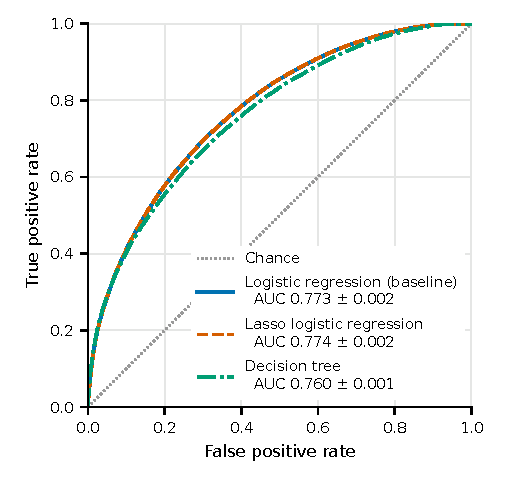
\includegraphics[width=0.5\linewidth]{figures/roc_oof.pdf}
  \caption{ROC curves from out-of-fold predictions on the training set. The
  legend gives each model's AUC as mean $\pm$ standard deviation over folds.
  The baseline and lasso curves overlap almost exactly.}
  \label{fig:roc}
\end{figure}

The baseline reaches a cross-validated AUC of 0.773, within the range
reported for admission-time models of similar outcomes, from 0.754 on triage
data \citep{zeleke2023} to 0.80--0.81 on the full health record
\citep{rajkomar2018}. Because our diagnosis features are coded at discharge,
this may overstate what a model could achieve on the day of admission. The
lasso is better than the baseline on every fold, but only by about 0.0003 AUC,
far less than the fold-to-fold standard deviation of 0.0017, so we treat the
two as tied. The pruned decision tree is clearly worse: its AUC is 0.013 lower
and its Brier score higher, and at the same cutoff it finds fewer long stays
(recall 0.66 against 0.70) at the same precision. All three models beat the
base-rate Brier score. Calibration curves, before and after recalibration,
will be added once every model has been fitted and recalibrated.

\section{Remaining work}
\label{sec:remaining}

\paragraph{Remaining sections.}
\begin{itemize}
  \item \textbf{Test-set results.} AUC and Brier score for every model, raw and
        after each recalibration, with bootstrap intervals and each model's
        difference from the baseline; a test-set ROC figure; precision and
        recall for context.
  \item \textbf{Calibration.} Out-of-fold calibration curves for every model,
        then test-set curves before and after Platt scaling and isotonic
        regression, and which models gained most from recalibration.
  \item \textbf{Fairness.} AUC, Brier score and calibration curves by payer and
        by race, with intervals, reported whether or not a gap appears.
  \item \textbf{Discussion and limitations.} What the comparison shows, including
        the possibility that flexible models do not beat logistic regression;
        diagnosis features coded at discharge; no patient identifier; a single
        random sample and seed; New York data for 2023--24 only.
  \item \textbf{Conclusion,} then acknowledgements with the AI use statement.
\end{itemize}

\paragraph{Experiments before Analysis Complete (30 November).}
\begin{itemize}
  \item 17--18 Nov: settle the gradient-boosted trees' grid, run its 5-fold
        refit, final fit and recalibration, and add it to
        Table~\ref{tab:cv} and Figure~\ref{fig:roc}.
  \item 19--22 Nov: tune, refit and recalibrate a random forest with a small
        grid.
  \item 23 Nov: decide whether to add an MLP; drop it if the random forest
        runs late.
  \item By 24 Nov: record the bootstrap design and the rule for choosing the
        recommended model before opening the test set.
  \item 25--26 Nov: score every model on the test set, once.
  \item 27--30 Nov: buffer; check figures against the saved results and freeze
        them. No new models after the test set is opened.
\end{itemize}

\begin{ack}
  % AI use statement (required by the course): name the assistants used and
  % what they were used for.
\end{ack}

% References. natbib is loaded by neurips_2026.sty; add entries to
% references.bib and cite with \citet / \citep.
\bibliographystyle{plainnat}
\bibliography{references}

% \appendix
% \section{...}

\end{document}
